\documentclass[ignorenonframetext,10pt,aspectratio=169]{beamer}

\usepackage{umut}
\usepackage{umuttr}
\usepackage[utf8]{inputenc}
\usepackage{uling}
\usepackage{uprog,usynsem}
\usepackage{fancyvrb}
\usepackage{natbib,unatbib}
\usepackage{linguex}
         \renewcommand{\refdash}{}
\usepackage{ubeamer}
\usepackage{verbatim}
\usepackage{graphicx}

\usepackage{tikz-qtree}
\usetikzlibrary{er,positioning}

\title{Higher order procedures: Part 2}
\author{\  \\ \vspace{20pt} Umut \"Ozge\\  }

\date{COGS 502: Symbols and Programming \\ METU, Informatics}

\begin{document}

\begin{frame}\frametitle{}
\thispagestyle{empty}
\maketitle
\end{frame}

\begin{frame}[t,plain]


\end{frame}

\begin{frame}[plain]
\begin{itemize}
\item Task: map a list of numbers to their factorials.
\pause
\item Task: take the procedure to use in mapping also as an argument. 
\end{itemize}
\end{frame}

\begin{frame}[t,plain]

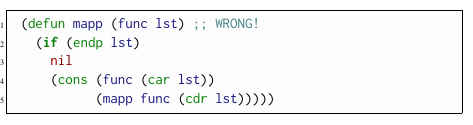
\includegraphics[scale=0.7]{img/mapp1.png}

\end{frame}

\begin{frame}[t,plain]
\Verb+FUNCALL+ wants its first argument to be something that would \emph{evaluate} to:
\begin{itemize}
\item[i.] a symbol with a function binding; or 
\item[ii.] a function.
\end{itemize}
\end{frame}


\begin{frame}[t,plain]

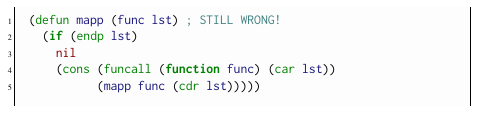
\includegraphics[scale=0.7]{img/mapp2.png}

\end{frame}

\begin{frame}[t,plain]

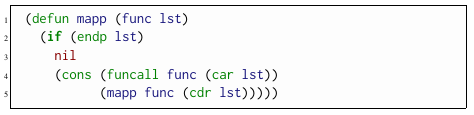
\includegraphics[scale=0.7]{img/mapp3.png}

\end{frame}

\end{document}
